\documentclass[]{scrreprt}%scrartcl
\usepackage{hyperref}
\usepackage{listings}
\usepackage[pdftex]{graphicx}
\usepackage[tablegrid]{vhistory}
\usepackage{acronym}
\usepackage{titling}
\usepackage{booktabs}
\usepackage{amssymb}
\usepackage{xcolor}
\usepackage[disable]{todonotes} %draft


%%%%%%%%%%%%%%%%%%%%%%%%%%%%%%%%%%%%%%%%%%%%%%%%%%%%%%%%%%%%%%%%%%%%%%

%% DOCUMENT SETUP

%%%%%%%%%%%%%%%%%%%%%%%%%%%%%%%%%%%%%%%%%%%%%%%%%%%%%%%%%%%%%%%%%%%%%%

%document title
\newcommand{\docTitle}{FABI3 - Flexible Assistive Button Interface}

%document workpackage number
%e.g.: AP x.x
\newcommand{\docWPNumber}{AP x.x}

%document status
%e.g.: Draft, Review or Final
\newcommand{\docStatus}{Review}

%document dissemination level
%PU....Public, RE....Restricted
\newcommand{\docDissemination}{PU}

%document ID
%e.g. TR-AP-X_X-YY, X_X -> workpackage, YY -> number
\newcommand{\docID}{functional$\_$requirements$\_$FABI}

%changelog / history
\newcommand{\docChangelog}{


  \vhEntry{0.1}{20.04.18}{BA}{Created}
  \vhEntry{0.2}{15.05.18}{BA}{Minor updates}
%  \vhEntry{0.3}{23.06.16}{TJ}{draft}
%  \vhEntry{0.7}{23.05.XX}{TJ}{draft}
%  \vhEntry{0.8}{23.05.XX}{TJ}{correction}
%  \vhEntry{0.9}{03.06.XX}{TJ}{Revised after review}
%  \vhEntry{1.0}{03.06.XX}{TJ}{Final version}

}


%%%%%%%%%%%%%%%%%%%%%%%%%%%%%%%%%%%%%%%%%%%%%%%%%%%%%%%%%%%%%%%%%%%%%%

%% GENERAL SETUP (NORMALLY NOT CHANGED)

%%%%%%%%%%%%%%%%%%%%%%%%%%%%%%%%%%%%%%%%%%%%%%%%%%%%%%%%%%%%%%%%%%%%%%

%%%% authors %%%%
\newcommand{\BA}{Benjamin Aigner}
\newcommand{\BAEmail}{beni}
\newcommand{\CV}{Chris Veigl}
\newcommand{\CVEmail}{chris}
%\newcommand{\TJ}{Thomas Jerabek}
%\newcommand{\TJEmail}{thomas.jerabek}
\newcommand{\note}[1]{\textcolor{black!50}{\textit{Note: #1}}}


%\usepackage{todonotes}
%
%\newcommand{\todoINFO}[1]{\todo[color=blue!25]{INFO: #1}}
%\newcommand{\todoIMPORTANT}[1]{\todo[color=red!25]{IMPORTANT: #1}}
%\newcommand{\todoREV}[1]{\todo[color=green!25]{REVIEWED: #1}}

\setlength\parindent{0pt}

\hypersetup{
	pdftitle  = {\docTitle},
	pdfkeywords = {\docTitle, Version \vhCurrentVersion from \vhCurrentDate},
	pdfauthor = {\vhAllAuthorsSet}
	}

%%%%%%%%%%%%%%%%%%%%%%%%%%%%%%%%%%%%%%%%%%%%%%%%%%%%%%%%%%%%%%%%%%%%%%

%% PREAMBLE PAGES

%%%%%%%%%%%%%%%%%%%%%%%%%%%%%%%%%%%%%%%%%%%%%%%%%%%%%%%%%%%%%%%%%%%%%%

\begin{document}
% 
% \title{ToRaDes - Technical Report \\ {\Huge \docTitle}}
% 
\includegraphics[height=20mm]{logo.png}
% \author{\vhListAllAuthorsLongWithAbbrev \\{University of Applied Sciences Technikum Wien}
% \\{H\"ochst\"adtplatz 6, A-1200 Vienna, Austria}
% \\{Email: {\texttt{\BAEmail, \TJEmail, \CVEmail}}}
% \\{\texttt{@technikum-wien.at}}}
% 
% \date{Version \vhCurrentVersion\ from \vhCurrentDate}
% \maketitle
% 
% \end{titlingpage}

\begin{titlepage}
	
	
\includegraphics[height=20mm]{logo.png} \hfill
	
\includegraphics[height=20mm]{fhtw.png}
	
	\centering
	\par\vspace{1cm}
	{\scshape\Huge ToRaDes \normalsize \par Toolbox for Rapid Development of Smart Homes and Assistive Technologies \par}
	\vspace{1cm}
	{\scshape\Large Requirements Specification\par}
	\vspace{1.5cm}
	{\huge\bfseries \docTitle \par}
	\vspace{2cm}
	{\Large
	\vhListAllAuthorsLongWithAbbrev \\{University of Applied Sciences Technikum Wien}
	\\{H\"ochst\"adtplatz 6, A-1200 Vienna, Austria}
	\\{Email: {\texttt{\BAEmail, \CVEmail}}}
	\\{\texttt{@asterics-foundation.org}}
	\par}
	\vfill
	{\large Version \vhCurrentVersion\ from \vhCurrentDate \par}
	\begin{flushright}
	 
\includegraphics[height=30mm]{ma23.png}
	\end{flushright}
\end{titlepage}

%Version history on bottom of page

\chapter*{Document Information}

\begin{tabular}{|l|l|}
\hline
\textbf{Issue Date} & \textbf{\vhCurrentDate}\\ \hline
%\textbf{Workpackage-Number} & \textbf{\docWPNumber}\\  \hline
\textbf{Status} & \textbf{\docStatus}\\  \hline
\textbf{Dissemination Level} & \textbf{\docDissemination} \\ \hline
\textbf{Document ID} & \textbf{\docID} \\ \hline
\end{tabular}

\section*{ToRaDes}
\textbf{Toolbox for Rapid Development of Smart Homes and Assistive Technologies} \\
This project has been funded by the Municipal Department 23 of the City of Vienna 
(Economic Affairs, Labour and Statistics - MA 23) in course of the 18th Call "Competence Teams for Research and Teaching".

\section*{AsTeRICS Foundation}

The AsTeRICS Foundation is a non-profit organisation that promotes the development and application of Open Source Assistive Technology (AT) for people with disabilities.

In course of several research projects, hardware- and software solutions have been developed at the University of Applied Sciences Technikum Wien, that can be easily adapted to individual needs and implemented at low cost. These solutions include devices for alternative computer input, augmentative and alternative communication (AAC) and environmental control systems – but also low-tech tools supporting activities of daily living. The AsTeRICS Foundation delivers these resources to users and other stakeholders.

\section*{Disclaimer}
The information in this document is provided as is and no guarantee or warranty is given that the information is fit for any particular purpose. The user thereof uses the information at its sole risk and liability. 

\vfill\nopagebreak
\parbox{\textwidth}{
\begin{versionhistory}
\docChangelog
\end{versionhistory}}
\clearpage

\tableofcontents
\clearpage


%%%%%%%%%%%%%%%%%%%%%%%%%%%%%%%%%%%%%%%%%%%%%%%%%%%%%%%%%%%%%%%%%%%%%%

%% DOCUMENT STARTS HERE

%%%%%%%%%%%%%%%%%%%%%%%%%%%%%%%%%%%%%%%%%%%%%%%%%%%%%%%%%%%%%%%%%%%%%%

\chapter{Introduction}

The FABI (Flexible Assistive Button Interface) allows control of a computer’s mouse cursor and
typing desired keyboard keys by using buttons and special/individual input methods. It can be
helpful for people who cannot use standard computer input devices – enabling them to play
games, surf the internet, write emails and much more.

\section{Purpose}

The FABI Interface can be actuated via dedicated buttons, momentary switches or self-made
electrical contacts. FABI consists of a hardware device and a graphical software application for configuration of
the desired functions.


\section{Scope}

This requirements specification is used to determine functional requirements (FR) and non-functional requirements (NFR) for FABI device.
The document is used in conjunction with the medical product classification and the risk management document.


\section{Background}

The AsTeRICS Foundation is a non-profit organisation that promotes the development and application of Open Source Assistive Technology (AT) for people with disabilities. Currently available button interfaces either lack of flexibility in context of configuration by the user or
in usability with many different platforms. In addition most of these assistive devices are very expensive.

FABI is designed as low-cost button interface, which can be bought as finished product or built in a DIY manner.


\section{References}

\note{Currently no references here.}


% \section{Assumptions and Constraints}
% 
% \note{Provide a list of contractual or task level assumptions and/or constraints that are preconditions to preparation of the FRS.  
% Assumptions are future situations beyond the control of the project, whose outcomes influence the success of a project.}
% 
% \subsection{Assumptions}
% \note{Examples of assumptions include: availability of a technical platform, legal changes and policy decisions.}
% 
% \subsection{Constraints}
% \note{
% Constraints are boundary conditions on how the system must be designed and constructed.  Examples include: legal requirements, technical standards, strategic decisions. 
% }
% \begin{itemize}
%  \item Constraints exist because of real business conditions.  For example, a delivery date is a constraint only if there are real business consequences that will happen as a result of not meeting the date.  
%  If failing to have the subject application operational by the specified date places the organization in legal default, the date is a constraint.
%  
%  \item Preferences are arbitrary.  For example, a date chosen arbitrarily is a preference.  Preferences, if included in the FRS, should be noted as such.
% \end{itemize}



%\section{Document Overview}

%\note{Provide a description of the document organization.}



% 
% \chapter{Methodology}
% 
% \note{Describe the overall approach used in the determination of the FRS contents.  Describe the modeling method(s) so non-technical readers can understand what they are conveying.}
% 


\chapter{Functional Requirements}

\section{Context}

The context of this requirement specification is limited to the FABI box (highlighted in green), a hardware module, and to the 
FABI software (FABIGUI, highlighted in blue) which is used to configure the FABI box.

\begin{center}
    \includegraphics[width=100mm]{context_diagram_FABI.png}
\end{center}


The external buttons are not scope of the FABI project, either they are bought off-the-shelf or they are built in a DIY manner. The PC which
is controlled by the FABI box is also not scope of this document.


\section{User Requirements}

\begin{description}
 \item[U1 - Compatibility] The FABI box should work with all major smartphone and PC platforms. This includes Microsoft Windows, Apple macOS, Linux, Apple iOS, Google Android. In addition, the IR remote part should work with most available consumer electronic devices, which can be controlled via IR remotes.
 \item[U2 - Input options] The FABI box should be able to trigger mouse, keyboard and joystick actions on the connected device.
 \item[U3 - Connections] This box should be connected either via a USB compatible interface or via a wireless Bluetooth connection.
 \item[U4 - Buttons] External buttons should be connected via a quasi-standard 3.5mm jack plug, which is used in nearly all available assistive buttons.
 \item[U5 - Configuration] The FABI box should store the configuration, which is used by the device itself with no further interaction necessary.
 \item[U6 - Configuration interface] The FABI box configuration should be configurable via two different possibilities: on the one hand, it should be compatible with previous FABI releases and their corresponding PC GUI. On the other hand, the FABI box itself should be able to provide a WiFi hotspot, which can be used to open a configuration page via a webbrowser.
 \item[U7 - Slots] The FABI box should be able to switch between different configurations, where the switching should be triggerable by the end user.
\end{description}


% \note{Provide requirements of the system, user or business, taking into account all major classes or categories of users.  
% Provide the type of security or other distinguishing characteristics of each set of users.  List the functional requirements that compose each user requirement.  
% As the functional requirements are decomposed, the highest level functional requirements are traced to the user requirements.  
% Inclusion of lower level functional requirements is not mandatory in the traceability to user requirements if the parent requirements are already traced to them.
% }
% \note{User requirement information can be in text or process flow format for each major user class that shows what inputs will initiate the system functions, system interactions, 
% and what outputs are expected to be generated by the system.  The scenarios should be comprehensive, to the extent that all user types and all major functions are covered.  
% Give each user requirement a unique number.  Typically, user requirements have a numbering system that is separate from the functional requirements.
% Requirements may be labeled with a leading U or other label indicating user requirements.}


\section{Data Flow Diagrams}

\begin{center}
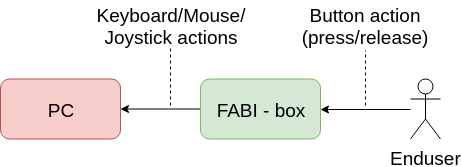
\includegraphics[width=100mm]{data_flow_fabi_normal.png} 
\end{center}

During normal operation, the enduser triggers actions be pressing (and releasing) the attached buttons. The button actions
are transformed to Keyboard, Mouse or Joystick actions (e.g., press left mouse button, click with left mouse buttonm, write a text,
press/release a joystick button), determined by the current configuration. The triggered action should transfer HID commands to the PC/smartphone device. 

These HID can be transferred either via a USB compatible interface or via a Bluetooth connection.

\begin{center}
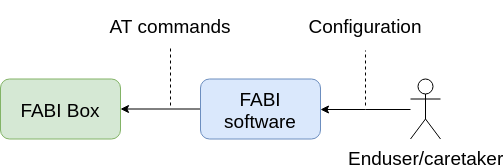
\includegraphics[width=100mm]{data_flow_fabi_config.png} 
\end{center}

If the user, a caretaker or any other authorized person needs to adapt the FABI configuration, two possibilities can be used:
\begin{description}
 \item[FABI software] This configuration GUI is used for all FABI devices (also previous versions 1 and 2). This software needs a USB connection, which is used to transfer so called \textit{AT commands} to the FABI device, which updates its configuration. The configuration
 user needs to connect the FABI box to his/her computer (this GUI is Microsoft Windows only), open the GUI, change the parameters and save it
 to the FABI box.
 \item[Web configuration] The FABI device is able to open a WiFi hotspot, to which a configurator can connect to. This WiFi hotspot is only
 enabled by a dedicated action, avoiding any unauthorized access. This configuration possibility is available for any WiFi device which has 
 a browser for opening the config page.
\end{description}



% \section{Logical Data Model/Data Dictionary}
% 
% \note{Create the initial Logical Data Model.  Describe data requirements by providing data entities, decomposition, and definitions in a data dictionary.
% The data requirements describe the business data needed by the application system.  
% Data requirements do not describe the physical database and are not at the level of identifying field names.}


\section{Functional Requirements}

%\note{List the functional requirements of the system.}

\subsection{Functional Requirements Group 1 - general}

General requirements overview.

\begin{table}[htb!]
 \centering
 \caption{Requirements Group 1 - general}
\label{req_group1}
 \begin{tabularx}{\textwidth}{|l|X|} \hline
 Section/\\ Requirement ID & Requirement definition\\ \hline  \hline
 FR1.0 & The device shall be able to translate button presses into Keyboard/Mouse/Joystick actions [U2][FR2]\\ \hline
 FR1.1 & The device shall be controlled via assistive buttons (connected via jack plugs) [U4][FR3]\\ \hline
 FR1.2 & The device shall be connected either by a cable or a wireless interface, using standardized interfaces [U3][FR4]\\ \hline
 FR1.3 & The device shall be able to store configuration on itself and switch between them [U5][U7][FR5]\\ \hline
 FR1.4 & The device shall be configured by either a PC GUI or a Web interface [U6][FR6]\\ \hline
 FR1.5 & The device shall be able to control consumer electronics via infrared commands [U1][FR7]\\ \hline
 FR1.6 & The device shall be able to work with: Linux, Apple macOS, Microsoft Windows, Android, iOS [U1]\\ \hline
 \end{tabularx}
\end{table}

\subsection{Functional Requirements Group 2 - Keyboard/Mouse/Joystick actions}

Requirements related to the output possibilities for triggering mouse, keyboard and joystick actions.

\begin{table}[htb!]
 \centering
 \caption{Requirements Group 2 - Keyboard/Mouse/Joystick actions}
\label{req_group2}
 \begin{tabularx}{\textwidth}{|l|X|} \hline
 Section/\\ Requirement ID & Requirement definition\\ \hline  \hline
 FR2.0 & The device shall be able to trigger a mouse left click\\ \hline
 FR2.1 & The device shall be able to trigger a mouse double left click\\ \hline
 FR2.2 & The device shall be able to trigger a mouse right click\\ \hline
 FR2.3 & The device shall be able to trigger a mouse middle click\\ \hline
 FR2.4 & The device shall be able to trigger a mouse wheel up/down\\ \hline
 FR2.5 & The device shall be able to change the mouse wheel steps\\ \hline
 FR2.6 & The device shall be able to move the mouse cursor in X and Y axis\\ \hline
 FR2.7 & The device shall be able to write an arbitrary text on the connected device \\ \hline
 FR2.8 & The device shall be able to press/release an arbitrary keyboard key\\ \hline
 FR2.9 & The device shall be able to set different joystick axis\\ \hline
 FR2.10 & The device shall be able to press/release different joystick buttons\\ \hline
 FR2.11 & The device shall be able to modify the joystick hat position\\ \hline
 \end{tabularx}
\end{table}

\subsection{Functional Requirements Group 3 - Button processing}

Button related requirements, defining the abilities for handling buttons.

\begin{table}[htb!]
 \centering
 \caption{Requirements Group 3 - Button processing}
\label{req_group3}
 \begin{tabularx}{\textwidth}{|l|X|} \hline
 Section/\\ Requirement ID & Requirement definition\\ \hline  \hline
 FR3.0 & The device shall be able to use standard off-the-shelf assistive buttons \\ \hline
 FR3.1 & The device shall be able to use DIY buttons \\ \hline
 FR3.2 & The device shall use a quasi-standard 3.5mm jack plug for button connections \\ \hline
 FR3.3 & The device shall be able to recognize a button press\\ \hline
 FR3.4 & The device shall be able to recognize a button release\\ \hline
 FR3.5 & The device shall be able to process a long button press\\ \hline
 FR3.6 & The device shall be able to have different delays for press, release and idle times (anti-tremor)\\ \hline
 \end{tabularx}
\end{table}
 

\subsection{Functional Requirements Group 4 - Interfaces}

Requirements related to the communication interfaces for normal operation (not configuring the device).

\begin{table}[htb!]
 \centering
 \caption{Requirements Group 4 - Interfaces}
\label{req_group4}
 \begin{tabularx}{\textwidth}{|l|X|} \hline
 Section/\\ Requirement ID & Requirement definition\\ \hline  \hline
 FR4.0 & The device shall use a USB compatible connection for a wired operation\\ \hline
 FR4.0.0 & The device shall use a USB-HID profile for highest possible compatibility\\ \hline
 FR4.0.1 & The device shall use a USB-CDC profile for configuration\\ \hline
 FR4.0.2 & The device shall implement a so-called composite device to support HID and CDC concurrently.\\ \hline
 FR4.0.2.0 & The device shall be able to switch on or off different parts of the HID profile, enabling maximum compatibility 
 to different specialized devices \\ \hline
 FR4.0.3 & The device shall be controlled via standardized AT commands\\ \hline
 FR4.0.4 & The device shall be able to trigger the same actions via buttons and via AT commands\\ \hline
 FR4.1 & The device shall use a Bluetooth LowEnergy connection for a wireless operation\\ \hline
 FR4.1.0 & The device shall use the HID-over-GATT (HOG) Bluetooth profile for triggering HID actions\\ \hline
 FR4.1.1 & The device shall implement the same HID commands for Bluetooth and USB\\ \hline
 FR4.2 & The device shall be powered via the USB compatible connection, even if in wireless mode.\\ \hline
 \end{tabularx}
\end{table}

\subsection{Functional Requirements Group 5 - Configurations (Slots)}

Requirements related to the handling of different configurations in so called slots.

\begin{table}[htb!]
 \centering
 \caption{Requirements Group 5 - Slots}
\label{req_group5}
 \begin{tabularx}{\textwidth}{|l|X|} \hline
 Section/\\ Requirement ID & Requirement definition\\ \hline  \hline
 FR5.0 & The device shall be able to store a minimum of 10 different configurations  \\ \hline
 FR5.1 & The device shall be able to modify the current configuration permanently \\ \hline
 FR5.2 & The device shall be able to modify the current configuration temporarily \\ \hline
 FR5.3 & The device shall be able to modify the configuration via the USB compatible interface \\ \hline
 FR5.4 & The device shall be able to modify the configuration via the WiFi interface  \\ \hline
 FR5.5 & The device shall be able to assign all meaningful actions to all input modalities  \\ \hline
 FR5.6 & The device shall store different properties into one configuration  \\ \hline
 FR5.6.0 & The device shall store an unique name for each configuration  \\ \hline
 FR5.6.1 & The device shall store the action for each triggered button (or any other input modality)  \\ \hline
 FR5.6.2 & The device shall store long press / idle times (anti-tremor settings) individually for each slot \\ \hline
 FR5.6.3 & The device shall store infrared commands independent from configuration settings \\ \hline
 %FR5.6.4 & The device shall store  \\ \hline
 %FR5.6.5 & The device shall store  \\ \hline
 FR5.7 & The device shall load a configuration by name  \\ \hline
 FR5.8 & The device shall load a configuration by navigating (next/previous)  \\ \hline
 FR5.9 & The device shall load a configuration by number  \\ \hline
 FR5.10 & The device shall be able to delete one, more or all configurations \\ \hline
 FR5.11 & The device shall be able to print out one or all configurations via USB compatible or WiFi interface \\ \hline
 \end{tabularx}
\end{table}


\subsection{Functional Requirements Group 6 - Infrared remotes}

Requirements related to infrared (IR) remote unit (receiving and transmitting)

\begin{table}[htb!]
 \centering
 \caption{Requirements Group 6 - Infrared remotes}
\label{req_group6}
 \begin{tabularx}{\textwidth}{|l|X|} \hline
 Section/\\ Requirement ID & Requirement definition\\ \hline  \hline
 FR6.0 & The device shall be able record usually used 38kHz infrared remote codes \\ \hline
 FR6.0.0 & The device shall be able to store at least 50 different remote codes \\ \hline 
 FR6.0.2 & The device shall be able to delete one, more or all IR commands (identified either by name or number) \\ \hline
 FR6.0.3 & The device shall be able to print the received IR command via USB compatible or WiFi interface \\ \hline
 FR6.1 & The device shall be able to replay previously recorded infrared remote sequences \\ \hline
 FR6.1.0 & A recorded IR code shall be replayed, identified by either a name or a number \\ \hline
 FR6.1.1 & The device shall be able to replay an arbitrary code sequence, with the same format as sent in FR6.0.3 \\ \hline
 \end{tabularx}
\end{table}

%\subsection{Functional Requirements Group 7 - Configuration Software}


\chapter{Other Requirements}

%\note{Describe the non-behavioral requirements.}

\section{Interface Requirements}

The main interface for this device is the USB compatible connection and/or the Bluetooth interface.
Due to the standardized interfaces and protocols, following documents are referenced here (this device shall implement these
referenced documents as they are an integral part of this document):

\begin{description}
 \item[Device Class Definition for Human Interface Devices (HID), v1.11] This document describes the necessary requirements for a USB HID compatible device. These specifications need to be implement within the firmware. USB low-level specifications are met by the used microcontroller.
 \item[Universal Serial Bus Class Definitions for Communications Devices, v1.2] This document specifies the interface for communicate via a virtual serial port over the USB compatible interface.
 \item[Bluetooth v4.2 core specification] This document specifies the Bluetooth interface. Implementation is provided by the selected microcontroller.
 \item[Bluetooth HID over GATT Profile, v1.0] Profile specification to tunnel HID commands over a Bluetooth connection. This profile is
 implemented by this device.
\end{description}

In addition to these standardized profiles/specifications, this device is implementing a command API, which is used to modify the configuration or control the device. The interface requirement is part of Doxygen documentation. The currently valid API is available in
this repository in \textit{$/docs/html/README\_\_AT\_\_command\_\_API\_8md.html$} (or in raw markdown: \textit{$/main/README\_AT\_command\_API.md$}).\\
\textbf{Note:} This AT command API is used for different devices. Please consult the documentation which commands are used for this device.\\
% 
% 
% \subsection{Hardware Interfaces}
% 
% \note{Define hardware interfaces supported by the system, including logical structure, physical addresses, and expected behavior.}
% 
% \subsection{Software Interfaces}
% 
% \note{Name the applications with which the subject application must interface.  State the following for each such application: name of application, external owner of application, 
% interface details (only if determined by the other application).
% It is acceptable to reference an interface control document for details of the interface interactions.}
% 
% \subsection{Communications Interfaces}
% 
% \note{Describe communications interfaces to other systems or devices, such as local area networks.}
% 
% 
% \section{Data Conversion Requirements}
% 
% \note{Describe the requirements needed for conversion of legacy data into the system.}
% 
% \section{Hardware/Software Requirements}
% 
% \note{Provide a description of the hardware and software platforms needed to support the system.}
% 
% 
% \section{Operational Requirements}
% 
% \note{
% Provide the operational requirements in this section.
% Do not state how these requirements will be satisfied.  For example, in the Reliability section, answer the question, 
% "How reliable must the system be"?  Do not state what steps will be taken to provide reliability.
% Distinguish preferences from requirements.  Requirements are based on business needs, preferences are not. 
% If, for example, the user requires a special response but does not have a business-related reason for it, that requirement is a preference.
% Other applicable requirements on system attributes may be added to the list of subsections below.]
% Operational requirements describe how the system will run and communicate with operations personnel.
% }
% 
% \subsection{Security and Privacy}
% 
% \note{
% Provide a list of the security requirements using the following criteria:
% }
% 
% \begin{itemize}
%  \item State the consequences of the following breaches of security in the subject application:
%     \begin{itemize}
%      \item Loss or corruption of data
%      \item Disclosure of secrets or sensitive information
%      \item Disclosure of privileged/privacy information about individuals
%      \item Corruption of software or introduction of malware, such as viruses
%     \end{itemize}
%   \item State the type(s) of security required. Include the need for the following as appropriate:
%     \begin{itemize}
%      \item Physical security.
%      \item Access by user role or types.
%      \item State access control requirements by data attribute.  For example, one group of users has permission to view an attribute but not update it while another group of users has permissions to update or view it.
%      \item State access requirements based on system function.  For example, if there is a need to grant access to certain system functions to one group of users, but not to another.  For example, "The system shall make Function X available to the System Administrator only".
%      \item State if there is a need for certification and accreditation of the security measures adopted for this application]
%     \end{itemize}
% \end{itemize}
% 
% \note{The Security Section describes the need to control access to the data. This includes controlling who may view and alter application data.}
% 
% \subsection{Audit Trail}
% 
% \note{List the activities recorded in the application’s audit trail. For each activity, list the data recorded.}
% 
% \subsection{Reliability}
% 
% \note{Reliability is the probability that the system processes work correctly and completely without being aborted.}
% 
% \begin{itemize}
%  \item State the following in this section:
%     \begin{itemize}
%      \item State the damage can result from failure of this system—indicate the criticality of the software, such as:
% 	\begin{itemize}
% 	 \item Loss of human life
% 	 \item Complete or partial loss of the ability to perform a mission-critical function
% 	 \item Loss of revenue
% 	 \item Loss of employee productivity
% 	\end{itemize}
%       \item What is the minimum acceptable level of reliability?
%     \end{itemize}
%     
%  \item State required reliability:
%     \begin{itemize}
%      \item Mean-Time-Between-Failure is the number of time units the system is operable before the first failure occurs.
%      \item Mean-Time-To-Failure is the number of time units before the system is operable divided by the number of failures during the time period.
%      \item Mean-Time-To-Repair is the number of time units required to perform system repair divided by the number of repairs during the time period.
%     \end{itemize}
% \end{itemize}
% 
% \subsubsection{Recoverability}
% 
% \note{Answer the following questions in this section:}
% \begin{itemize}
%  \item In the event the application is unavailable to users (down) because of a system failure, how soon after the failure is detected must function be restored?
%  \item In the event the database is corrupted, to what level of currency must it be restored?  For example “The database must be capable of being restored to its condition of no more than 1 hour before the corruption occurred”.
%  \item If the processing site (hardware, data, and onsite backup) is destroyed, how soon must the application be able to be restored?]
% \end{itemize}
% \note{Recoverability is the ability to restore function and data in the event of a failure.}
% 
% \subsubsection{System availability}
% 
% \note{State the period during which the application must be available to users.  
% For example, "The application must be available to users Monday through Friday between the hours of 6:30 a.m. and 5:30 p.m. EST."
% If the application must be available to users in more than one time zone, state the earliest start time and the latest stop time. Consider daylight savings time, too.
% Include use peak times.  These are times when system unavailability is least acceptable.
% System availability is the time when the application must be available for use.  Required system availability is used in determining when maintenance may be performed.}
% 
% \subsubsection{General Performance}
% 
% \note{Specific performance requirements, related to a specific functional requirement, should be listed with that functional requirement.
% Describe the requirements for the following:}
% \begin{itemize}
%  \item Response time for queries and updates
%  \item Throughput
%  \item Expected rate of user activity (for example, number of transactions per hour, day, or month, or cyclical periods)
% \end{itemize}
% 
% \subsubsection{Capacity}
% 
% \note{List the required capacities and expected volumes of data in business terms.  
% Do not state capacities in terms of system memory requirements or disk space - if growth trends or projections are available, provide them.}
% 
% \subsubsection{Data Retention}
% 
% \note{Describe the length of time various forms of data must be retained and the requirements for its destruction.
% For example, “The system shall retain application information for 3 years”.  Different forms of data include: system documentation, audit records, database records, access records.}
% 
% \subsubsection{Error Handling}
% 
% \note{Describe system error handling.}
% 
% \subsubsection{Validation Rules}
% 
% \note{Describe system validation rules.}
% 
% \subsubsection{Conventions/Standards}
% 
% \note{Describe system conventions and standards followed.\\
% For example: Microsoft standards are followed for windows, Institute of Electrical and Electronics Engineers (IEEE) for data formats, etc.}

\chapter{Glossary}

 \begin{tabularx}{\textwidth}{|l|X|} \hline
 \textbf{AT (commands)}   &   Serial command API, starting each command with text sequence ``AT''\\ \hline
 \textbf{AT}    &   Assistive Technology \\ \hline
 \textbf{API}   &   Application Programming Interface      \\ \hline
 \textbf{CDC}   &   Class Definition for Communications (USB specification) \\ \hline
 \textbf{ESP32} &   Application processor by Espressif \\ \hline
 \textbf{FABI}  &   Flexible Assistive Button Interface \\ \hline
 \textbf{GATT}  &   Generic Attributes (Bluetooth Low Energy services) \\ \hline
 \textbf{HID}   &   Human Interface Device      \\ \hline
 \textbf{HOG}   &   HID over GATT (Bluetooth profile) \\ \hline
 \textbf{IEEE}  &   Institute of Electrical and Electronics Engineers \\ \hline
 \textbf{USB}   &   Universal Serial Bus \\ \hline
 \textbf{WiFi}  &   Synonym for wireless networking based on IEEE 802.11 \\ \hline
 \end{tabularx}


\end{document}
